\chapter{Results}

\FloatBarrier

\section{Graph-aware prompting improves F1, precision, and recall}

RQ1 is answered by the three within-model contrasts. Figure~\ref{figure:7.1} shows paired-cohort F1 values, and Table~\ref{table:A.4} reports per-seed graph minus no-graph effects and intervals. All twelve F1 effects are positive, including each of the three Llama seeds. The treatment includes graph evidence and its interpretation instructions.


\begin{figure}[htbp]
\centering
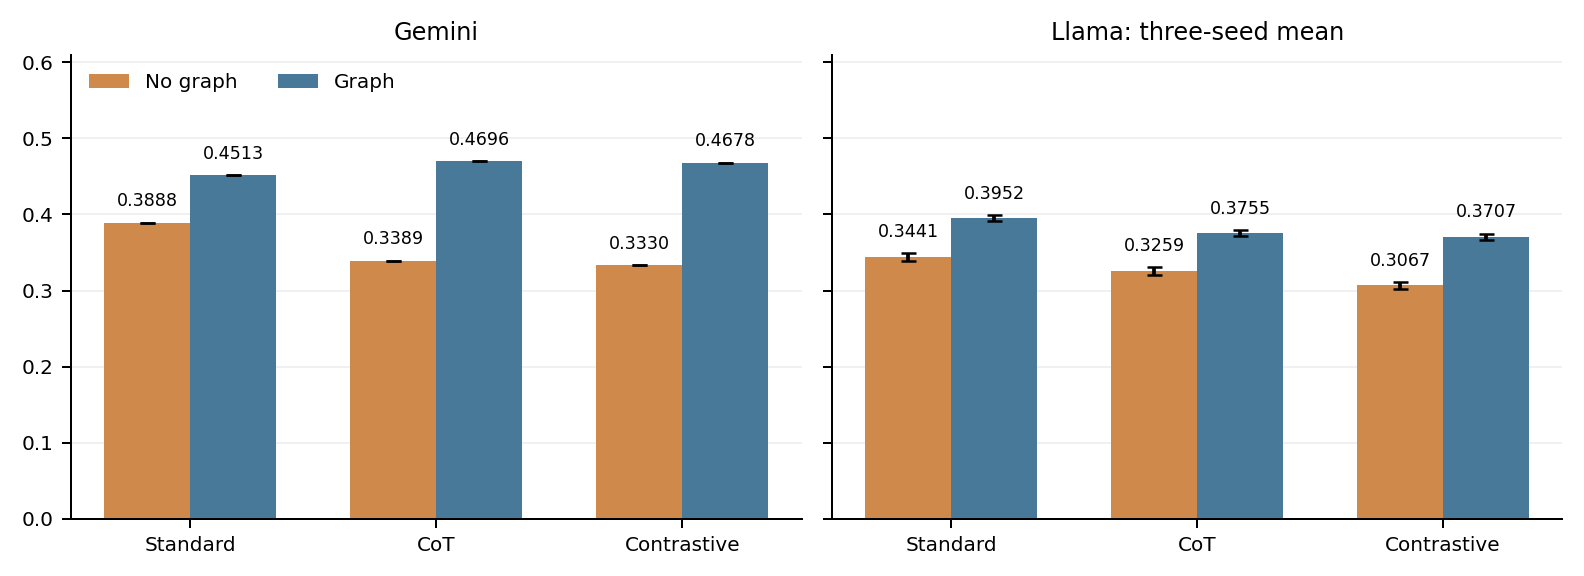
\includegraphics[width=\linewidth]{figures/f1.png}
\caption{Mean entity F1 on each matched graph/no-graph cohort; Gemini and the Llama seed mean; error bars show sample SD across three seed means. Paired effects and n are in Table~\ref{table:A.4}.}\label{figure:7.1}
\end{figure}

Parents expose broader category vocabulary and neighbours constrain the intended branch, which can improve both selecting and ordering labels. These are plausible explanations, not isolated causal mechanisms: the added graph note and worked-example wording also contribute to the treatment.


\subsection*{Precision, recall, and description overlap}

Table~\ref{table:7.1} reports precision, recall, and generated-label counts. Llama means use the same entities across all three seeds and both conditions within each style.


\begingroup
\begin{table}[!htbp]
\setlength{\tabcolsep}{3pt}
\renewcommand{\arraystretch}{1.18}
\fontsize{8.5}{10.5}\selectfont
\renewcommand{\thetable}{7.1}
\caption{Precision, recall, and generated labels; N/G denote no graph/graph.}\label{table:7.1}
\begin{tabular}{>{\raggedright\arraybackslash}p{\dimexpr 0.254902\linewidth-2\tabcolsep\relax}>{\raggedright\arraybackslash}p{\dimexpr 0.117647\linewidth-2\tabcolsep\relax}>{\raggedright\arraybackslash}p{\dimexpr 0.117647\linewidth-2\tabcolsep\relax}>{\raggedright\arraybackslash}p{\dimexpr 0.117647\linewidth-2\tabcolsep\relax}>{\raggedright\arraybackslash}p{\dimexpr 0.117647\linewidth-2\tabcolsep\relax}>{\raggedright\arraybackslash}p{\dimexpr 0.137255\linewidth-2\tabcolsep\relax}>{\raggedright\arraybackslash}p{\dimexpr 0.137255\linewidth-2\tabcolsep\relax}}
\toprule
\textbf{Model/style} & \textbf{P N} & \textbf{P G} & \textbf{R N} & \textbf{R G} & \textbf{Labels N} & \textbf{Labels G} \\
\midrule
Gemini Standard & 0.4714 & 0.5628 & 0.3503 & 0.3968 & 8.3930 & 8.0630 \\
Gemini CoT & 0.4740 & 0.6116 & 0.2782 & 0.4000 & 6.6190 & 7.4150 \\
Gemini Contrastive & 0.4708 & 0.6120 & 0.2704 & 0.3969 & 6.4840 & 7.3540 \\
Llama mean Standard & 0.3961 & 0.4651 & 0.3391 & 0.3767 & 10.8184 & 9.7018 \\
Llama mean CoT & 0.3710 & 0.4296 & 0.3191 & 0.3677 & 9.9455 & 10.0369 \\
Llama mean Contrastive & 0.3536 & 0.4367 & 0.2959 & 0.3539 & 9.7305 & 9.5712 \\
\bottomrule
\end{tabular}
\end{table}
\endgroup


Precision and recall improve together in all twelve primary contrasts, so list expansion alone does not explain the gains. Figure~\ref{figure:7.2} shows that standard graph outputs are shorter. Gemini CoT lists grow from 6.619 to 7.415 labels (+0.796), and contrastive lists from 6.484 to 7.354 (+0.870), whereas standard lists shrink by 0.330. Explanation-bearing gains therefore combine greater coverage with improved precision. Counts retain repetitions; set scoring deduplicates normalized labels.


\begin{figure}[htbp]
\centering
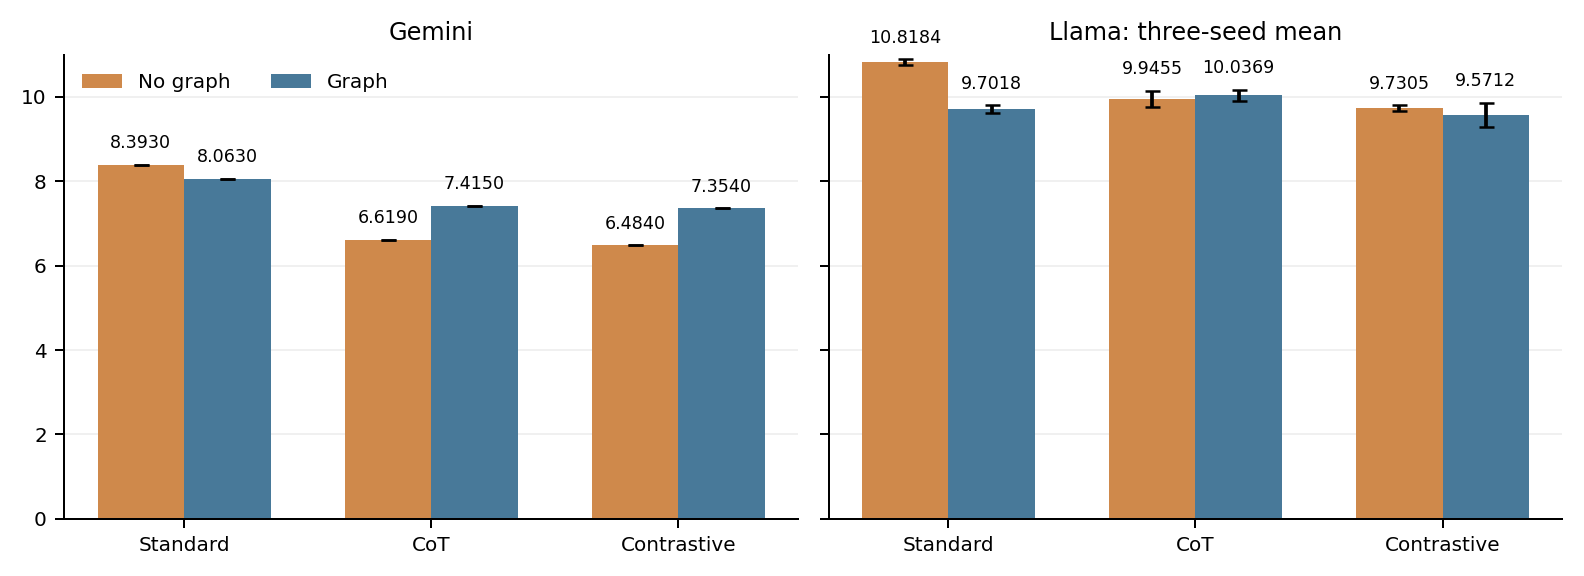
\includegraphics[width=\linewidth]{figures/length.png}
\caption{Mean generated type-label count on matched cohorts; Llama error bars are the SD of three seed means.}\label{figure:7.2}
\end{figure}

Table~\ref{table:7.2} separates effects according to literal centre-label occurrence in the description.


\begingroup
\begin{table}[!htbp]
\setlength{\tabcolsep}{3pt}
\renewcommand{\arraystretch}{1.18}
\fontsize{8.5}{10.5}\selectfont
\renewcommand{\thetable}{7.2}
\caption{Paired F1 gains by literal centre-label occurrence in the description.}\label{table:7.2}
\begin{tabular}{>{\raggedright\arraybackslash}p{\dimexpr 0.355120\linewidth-2\tabcolsep\relax}>{\raggedright\arraybackslash}p{\dimexpr 0.161220\linewidth-2\tabcolsep\relax}>{\raggedright\arraybackslash}p{\dimexpr 0.161220\linewidth-2\tabcolsep\relax}>{\raggedright\arraybackslash}p{\dimexpr 0.161220\linewidth-2\tabcolsep\relax}>{\raggedright\arraybackslash}p{\dimexpr 0.161220\linewidth-2\tabcolsep\relax}}
\toprule
\textbf{Model/style} & \textbf{Present n} & \textbf{Gain} & \textbf{Absent n} & \textbf{Gain} \\
\midrule
Gemini Standard & 265 & +0.0591 & 735 & +0.0637 \\
Gemini CoT & 265 & +0.0967 & 735 & +0.1431 \\
Gemini Contrastive & 265 & +0.1095 & 735 & +0.1439 \\
Llama 0 Standard & 265 & +0.0537 & 735 & +0.0615 \\
Llama 0 CoT & 265 & +0.0395 & 734 & +0.0599 \\
Llama 0 Contrastive & 263 & +0.0524 & 732 & +0.0642 \\
Llama 42 Standard & 265 & +0.0558 & 733 & +0.0454 \\
Llama 42 CoT & 260 & +0.0394 & 731 & +0.0499 \\
Llama 42 Contrastive & 264 & +0.0650 & 727 & +0.0606 \\
Llama 123 Standard & 263 & +0.0365 & 734 & +0.0482 \\
Llama 123 CoT & 263 & +0.0589 & 732 & +0.0435 \\
Llama 123 Contrastive & 263 & +0.0582 & 732 & +0.0737 \\
\bottomrule
\end{tabular}
\end{table}
\endgroup


The gains in the label-absent group directly address the running-example concern: graph-aware prompting is useful beyond descriptions that literally name the selected centre. This split is descriptive, because lexical overlap also co-varies with entity categories, gold-list length, and available context.


Table~\ref{table:A.4} reports helped, tied, and harmed counts for all twelve style/run contrasts. A positive mean does not imply a benefit for every entity.


\FloatBarrier

\section{Variation across the three Llama seeds}

The three seeds assess the stability of the Llama results supporting RQ1 and RQ4. Table~\ref{table:7.3} uses one common completed cohort per condition, so seed variation is not caused by different entity membership. The standard graph condition has the largest F1 among the three combined-graph styles at every seed, while the relation-only results vary more.


\begingroup
\begin{table}[!htbp]
\setlength{\tabcolsep}{3pt}
\renewcommand{\arraystretch}{1.18}
\fontsize{8.5}{10.5}\selectfont
\renewcommand{\thetable}{7.3}
\caption{Llama F1 variability on common completed entities; sample SD across three seed means.}\label{table:7.3}
\begin{tabular}{>{\raggedright\arraybackslash}p{\dimexpr 0.607843\linewidth-2\tabcolsep\relax}>{\raggedright\arraybackslash}p{\dimexpr 0.196078\linewidth-2\tabcolsep\relax}>{\raggedright\arraybackslash}p{\dimexpr 0.196078\linewidth-2\tabcolsep\relax}}
\toprule
\textbf{Condition} & \textbf{n} & \textbf{SD} \\
\midrule
Standard no graph & 1000 & 0.0047 \\
Standard graph & 995 & 0.0039 \\
CoT no graph & 994 & 0.0053 \\
CoT graph & 991 & 0.0039 \\
Contrastive no graph & 991 & 0.0046 \\
Contrastive graph & 990 & 0.0041 \\
Parents only & 997 & 0.0218 \\
Siblings only & 993 & 0.0119 \\
Children only & 997 & 0.0160 \\
\bottomrule
\end{tabular}
\end{table}
\endgroup


Parent-only F1 is more variable than the combined standard graph result. It exceeds the combined-context F1 at seeds 0 and 42 but falls below it at seed 123. Combined context supplies several kinds of evidence, which may reduce dependence on an individual relation list; parent-only responses can instead be more sensitive to sampled choices of broad labels. This is a possible explanation for the observed variability, not a tested mechanism. The stable combined-style ordering supports that comparison more strongly than selecting one best relation condition from a single seed.


With failures assigned zero across all 1,000 entities, all nine Llama graph gains remain positive, from +0.0437 to +0.0702. Incomplete outputs do not change the direction of RQ1, although accepted-response means remain conditional on validation and retries.


\FloatBarrier

\section{Maximum-depth gold-label ranking and graded list quality}

RQ1 also concerns ranked output. Figure~\ref{figure:7.3} shows MRR, and Table~\ref{table:7.4} gives paired gains in MRR and nDCG. Both increase in every model-by-style contrast. Gemini’s ranking gains are larger than Llama’s, especially under the explanation-bearing templates.


\begin{figure}[htbp]
\centering
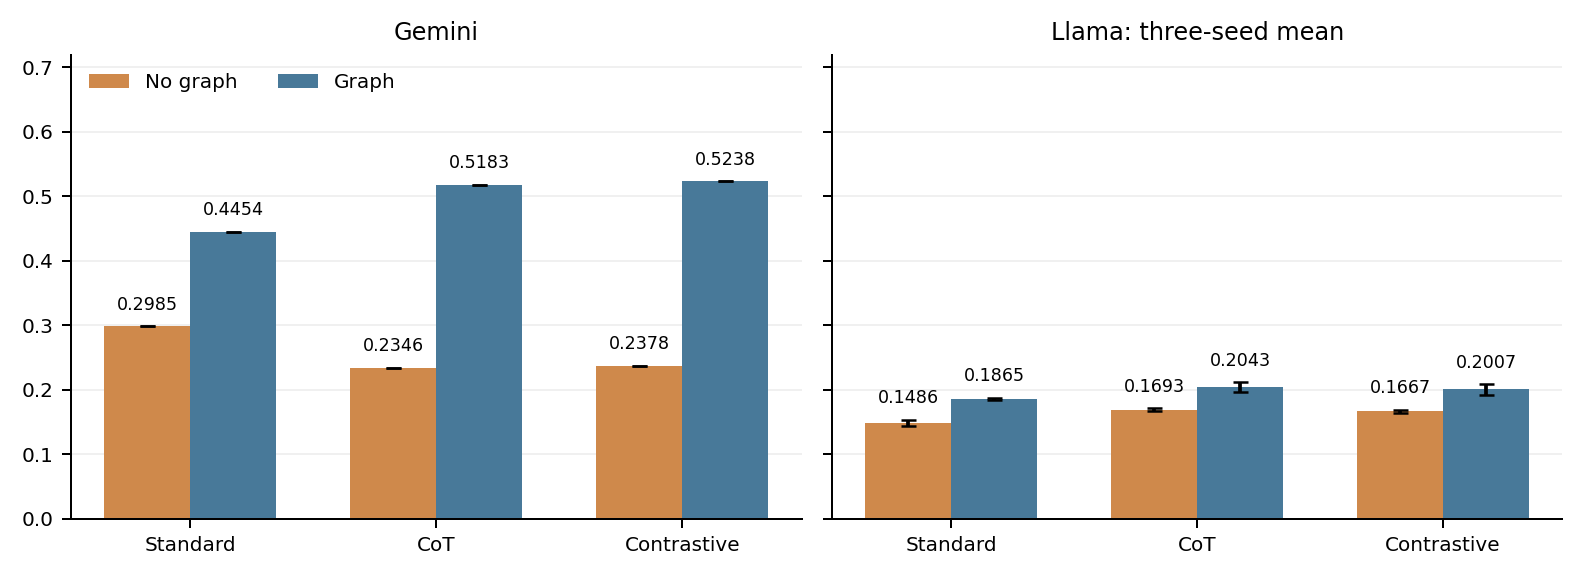
\includegraphics[width=\linewidth]{figures/mrr.png}
\caption{Maximum-depth gold-label MRR, using matched successful responses. Llama is summarized by the three-seed mean with sample SD.}\label{figure:7.3}
\end{figure}

\begingroup
\begin{table}[!htbp]
\setlength{\tabcolsep}{3pt}
\renewcommand{\arraystretch}{1.18}
\fontsize{8.5}{10.5}\selectfont
\renewcommand{\thetable}{7.4}
\caption{Paired graph gains in MRR and depth-weighted nDCG.}\label{table:7.4}
\begin{tabular}{>{\raggedright\arraybackslash}p{\dimexpr 0.542484\linewidth-2\tabcolsep\relax}>{\raggedright\arraybackslash}p{\dimexpr 0.228758\linewidth-2\tabcolsep\relax}>{\raggedright\arraybackslash}p{\dimexpr 0.228758\linewidth-2\tabcolsep\relax}}
\toprule
\textbf{Model/style} & \textbf{MRR gain} & \textbf{nDCG gain} \\
\midrule
Gemini Standard & +0.1469 & +0.1423 \\
Gemini CoT & +0.2837 & +0.2319 \\
Gemini Contrastive & +0.2860 & +0.2342 \\
Llama 0 Standard & +0.0402 & +0.1353 \\
Llama 0 CoT & +0.0281 & +0.1257 \\
Llama 0 Contrastive & +0.0439 & +0.1288 \\
Llama 42 Standard & +0.0445 & +0.1384 \\
Llama 42 CoT & +0.0440 & +0.1315 \\
Llama 42 Contrastive & +0.0309 & +0.1271 \\
Llama 123 Standard & +0.0304 & +0.1302 \\
Llama 123 CoT & +0.0329 & +0.1198 \\
Llama 123 Contrastive & +0.0261 & +0.1289 \\
\bottomrule
\end{tabular}
\end{table}
\endgroup


Table~\ref{table:A.2} reports maximum-depth hit rate, rank bins, strict accuracy, micro-F1, hierarchical F1, and hierarchy consistency. Table~\ref{table:A.3} reports error distance and direction, with explicit denominators. These diagnostics distinguish recovering labels, ranking them early, and generating an ancestor-closed list.


For standard prompting, maximum-depth hit rate rises from 0.4200 to 0.5930 for Gemini and from 0.1850 to 0.2610 for Llama seed 0 (Table~\ref{table:A.2b}). Exact reconstruction remains rare: strict accuracy is 0.0010 in both Gemini conditions and zero in both Llama seed-0 conditions. Hierarchy consistency falls from 0.3282 to 0.2380 for Gemini and from 0.5479 to 0.4298 for Llama seed 0, despite higher hierarchical F1 (Table~\ref{table:A.2a}). Closer ancestor-augmented agreement therefore does not imply a more explicitly closed output list.


Llama’s nDCG gain is consistently larger than its MRR gain. This is consistent with recovering or ordering intermediate gold classes more successfully than recovering a maximum-depth label early. The graph can supply broad vocabulary directly, while identifying the omitted centre still requires interpreting the description and relations. These output patterns do not establish an internal reasoning route.


Selecting a best prompt depends on the metric. The standard graph prompt leads Llama’s combined-context F1 across seeds, while its maximum-depth ranking can favour an explanation-bearing condition. Gemini’s CoT and contrastive graph scores are close; their small differences should not be treated as a general superiority claim.


\FloatBarrier

\section{Relation ablations and model comparison}

RQ2 and H1 concern the relative usefulness of relation conditions. Table~\ref{table:7.5} reports paired gains over standard no graph; full condition scores are in Table~\ref{table:A.1}. Parent-only F1 exceeds sibling-only F1 for Gemini and all Llama seeds, so H1 is not supported. Combined standard context exceeds every single-relation condition for Gemini, but not for Llama seeds 0 and 42.


\begingroup
\begin{table}[!htbp]
\setlength{\tabcolsep}{3pt}
\renewcommand{\arraystretch}{1.18}
\fontsize{8.5}{10.5}\selectfont
\renewcommand{\thetable}{7.5}
\caption{Paired standard-style F1 gains over no graph.}\label{table:7.5}
\begin{tabular}{>{\raggedright\arraybackslash}p{\dimexpr 0.311547\linewidth-2\tabcolsep\relax}>{\raggedright\arraybackslash}p{\dimexpr 0.172113\linewidth-2\tabcolsep\relax}>{\raggedright\arraybackslash}p{\dimexpr 0.172113\linewidth-2\tabcolsep\relax}>{\raggedright\arraybackslash}p{\dimexpr 0.172113\linewidth-2\tabcolsep\relax}>{\raggedright\arraybackslash}p{\dimexpr 0.172113\linewidth-2\tabcolsep\relax}}
\toprule
\textbf{Condition} & \textbf{Gemini} & \textbf{Llama 0} & \textbf{Llama 42} & \textbf{Llama 123} \\
\midrule
Parents only & +0.0414 & +0.0638 & +0.0598 & +0.0213 \\
Siblings only & +0.0070 & +0.0024 & +0.0162 & +0.0014 \\
Children only & +0.0272 & +0.0119 & +0.0204 & -0.0092 \\
Standard graph & +0.0625 & +0.0594 & +0.0482 & +0.0451 \\
\bottomrule
\end{tabular}
\end{table}
\endgroup


Parent labels often belong to the gold ancestor chain, so their utility includes direct access to broader valid vocabulary. Siblings generally do not provide that same immediate overlap. Differences in relation availability and context size also matter. The ablations therefore identify useful prompt configurations rather than proving that parent edges are intrinsically superior in every setting.


Sibling-only context can still assist the more specific ranking task: Gemini’s sibling-only MRR is 0.4316, compared with 0.2985 without graph. A relation may aid identifying a particular class without recovering enough of the broader gold hierarchy to maximize F1.


\begingroup
\begin{table}[!htbp]
\setlength{\tabcolsep}{3pt}
\renewcommand{\arraystretch}{1.18}
\fontsize{8.5}{10.5}\selectfont
\renewcommand{\thetable}{7.6}
\caption{Empty-child partial control: children-only minus standard no graph on entities without test child context.}\label{table:7.6}
\begin{tabular}{>{\raggedright\arraybackslash}p{\dimexpr 0.196078\linewidth-2\tabcolsep\relax}>{\raggedright\arraybackslash}p{\dimexpr 0.076253\linewidth-2\tabcolsep\relax}>{\raggedright\arraybackslash}p{\dimexpr 0.152505\linewidth-2\tabcolsep\relax}>{\raggedright\arraybackslash}p{\dimexpr 0.152505\linewidth-2\tabcolsep\relax}>{\raggedright\arraybackslash}p{\dimexpr 0.141612\linewidth-2\tabcolsep\relax}>{\raggedright\arraybackslash}p{\dimexpr 0.281046\linewidth-2\tabcolsep\relax}}
\toprule
\textbf{Model} & \textbf{n} & \textbf{Standard} & \textbf{Child-only} & \textbf{Gain} & \textbf{95\% interval} \\
\midrule
Gemini & 549 & 0.3840 & 0.4084 & +0.0243 & [+0.0160, +0.0331] \\
Llama 0 & 549 & 0.3352 & 0.3485 & +0.0133 & [+0.0014, +0.0255] \\
Llama 42 & 548 & 0.3452 & 0.3622 & +0.0170 & [+0.0059, +0.0287] \\
Llama 123 & 548 & 0.3367 & 0.3417 & +0.0049 & [-0.0067, +0.0171] \\
\bottomrule
\end{tabular}
\end{table}
\endgroup


Table~\ref{table:7.6} shows small positive point estimates, approximately +0.005 to +0.024, but the Llama seed-123 interval includes zero and seed 0 only narrowly excludes it. This is suggestive evidence of a template contribution, not a uniformly established positive instruction effect. Gemini’s effect is about +0.02 compared with its +0.0625 full-cohort standard graph gain. Because the cohorts and prompt changes differ, this is an indicative comparison, not an estimate of the fraction attributable to the template.


The test child lists are empty for these 549 entities. The comparison measures the empty-evidence prompt package, which still changes graph instructions and the demonstration. It therefore helps assess instruction/template effects but does not isolate the graph note alone. The full graph gains should not be attributed entirely to structural evidence.


RQ4 compares Gemini with each Llama seed on shared completed entities, condition by condition. Table~\ref{table:7.7} summarizes Gemini minus Llama F1 averaged over seeds; Table~\ref{table:A.5} gives every per-seed interval and model difference in graph gains. Positive values favour Gemini; all nine conditions favour Gemini against each seed. This is a comparison of the recorded systems, including Gemini’s default internal thinking, not a controlled test of model architecture.


\begingroup
\begin{table}[!htbp]
\setlength{\tabcolsep}{3pt}
\renewcommand{\arraystretch}{1.18}
\fontsize{8.5}{10.5}\selectfont
\renewcommand{\thetable}{7.7}
\caption{Gemini minus the mean of three Llama seeds, on common completed entities.}\label{table:7.7}
\begin{tabular}{>{\raggedright\arraybackslash}p{\dimexpr 0.389978\linewidth-2\tabcolsep\relax}>{\raggedright\arraybackslash}p{\dimexpr 0.087146\linewidth-2\tabcolsep\relax}>{\raggedright\arraybackslash}p{\dimexpr 0.217865\linewidth-2\tabcolsep\relax}>{\raggedright\arraybackslash}p{\dimexpr 0.305011\linewidth-2\tabcolsep\relax}}
\toprule
\textbf{Condition} & \textbf{n} & \textbf{F1 difference} & \textbf{95\% interval} \\
\midrule
Standard no graph & 1000 & +0.0443 & [+0.0367, +0.0520] \\
Standard graph & 995 & +0.0556 & [+0.0468, +0.0649] \\
CoT no graph & 994 & +0.0131 & [+0.0056, +0.0211] \\
CoT graph & 991 & +0.0949 & [+0.0857, +0.1042] \\
Contrastive no graph & 991 & +0.0264 & [+0.0199, +0.0333] \\
Contrastive graph & 990 & +0.0970 & [+0.0886, +0.1053] \\
Parents only & 997 & +0.0377 & [+0.0294, +0.0458] \\
Siblings only & 993 & +0.0450 & [+0.0359, +0.0539] \\
Children only & 997 & +0.0640 & [+0.0552, +0.0727] \\
\bottomrule
\end{tabular}
\end{table}
\endgroup


Gemini graph prompts use about 1.8, 2.7, and 3.0 times as many thinking tokens as their no-graph counterparts for standard, CoT, and contrastive styles (Table~\ref{table:5.1}). These ratios follow the same ordering as the F1 gains of 0.0625, 0.1308, and 0.1348. More structural evidence therefore coincides with more internal computation. The experiment does not hold the thinking budget fixed, so it cannot separate their contributions; the association across three styles does not show that additional thinking causes the gains.


Gemini’s standard F1 gain is comparable to Llama seed 0, but its explanation-bearing graph gains are substantially larger than those of all three Llama seeds. Thus absolute model advantage and response to graph evidence remain distinct observations.


\FloatBarrier

\section{The matched child-removal experiment}

This ablation addresses the child component of RQ2. An all-entity children-only average mixes informative child lists with 549 empty lists, so it cannot show what changes when existing child context is removed. The matched experiment instead compares the same eligible entities and retains parents, siblings, and prompting style, while removing the child section and child-specific instructions.


\begin{figure}[htbp]
\centering
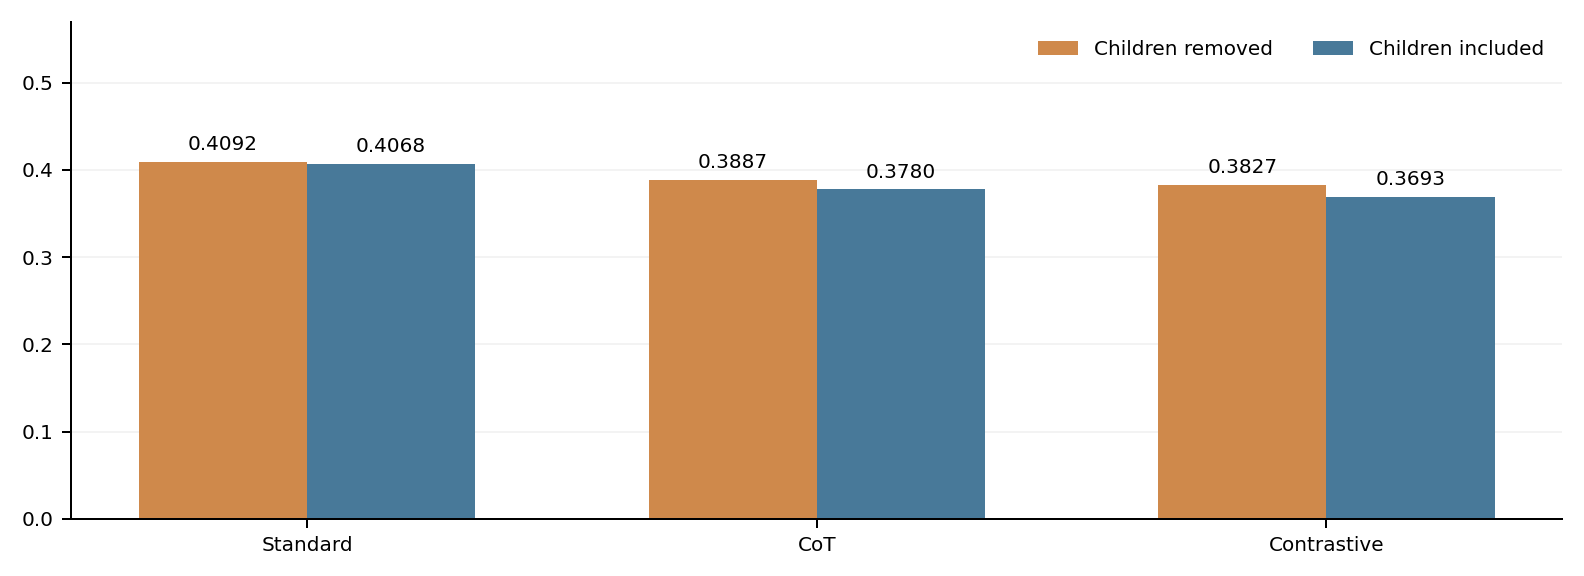
\includegraphics[width=\linewidth]{figures/child.png}
\caption{Llama seed 0 child-removal comparison on matched successful responses.}\label{figure:7.4}
\end{figure}

\begingroup
\begin{table}[!htbp]
\setlength{\tabcolsep}{3pt}
\renewcommand{\arraystretch}{1.18}
\fontsize{8.5}{10.5}\selectfont
\renewcommand{\thetable}{7.8}
\caption{Llama seed 0: paired child effects on F1: included minus removed.}\label{table:7.8}
\begin{tabular}{>{\raggedright\arraybackslash}p{\dimexpr 0.196078\linewidth-2\tabcolsep\relax}>{\raggedright\arraybackslash}p{\dimexpr 0.076253\linewidth-2\tabcolsep\relax}>{\raggedright\arraybackslash}p{\dimexpr 0.152505\linewidth-2\tabcolsep\relax}>{\raggedright\arraybackslash}p{\dimexpr 0.152505\linewidth-2\tabcolsep\relax}>{\raggedright\arraybackslash}p{\dimexpr 0.141612\linewidth-2\tabcolsep\relax}>{\raggedright\arraybackslash}p{\dimexpr 0.281046\linewidth-2\tabcolsep\relax}}
\toprule
\textbf{Style} & \textbf{n} & \textbf{Removed} & \textbf{Included} & \textbf{Effect} & \textbf{95\% interval} \\
\midrule
Standard & 451 & 0.4092 & 0.4068 & -0.0024 & [-0.0165, +0.0115] \\
CoT & 450 & 0.3887 & 0.3780 & -0.0108 & [-0.0256, +0.0038] \\
Contrastive & 448 & 0.3827 & 0.3693 & -0.0134 & [-0.0286, +0.0019] \\
\bottomrule
\end{tabular}
\end{table}
\endgroup


Figure~\ref{figure:7.4} and Table~\ref{table:7.8} show small negative point estimates in all three styles, but all three intervals include zero. These data establish neither a clear F1 benefit nor a clear F1 harm from including children. Under standard prompting, recall increases by 0.0176 and MRR by 0.0282, while precision falls by 0.0463 and hierarchical F1 by 0.0233. Narrower neighbours may help identify a class but also encourage additional unsupported specificity or a different broader hierarchy.


The planned cohort contains 451 entities. Completed pairs number 451 for standard, 450 for CoT, and 448 for contrastive: one child-removal CoT output and three eligible main contrastive outputs are incomplete. The matched denominators avoid treating those missing outputs as valid responses.


The experimental scope is a matched child-context intervention for Llama 3.1 8B Instruct at seed 0, across the three prompting styles and the 451 child-eligible entities. It measures the effect of the implemented child-removal treatment within this setting; cross-model comparisons are provided by the main nine-condition experiments.


\FloatBarrier

\section{Effects across taxonomy depth}

RQ3 and H2 concern whether graph benefit increases with depth. The maximum annotated-depth groups 4–5, 6–7, and 8+ contain 198, 465, and 337 entities before completion filtering. Table~\ref{table:7.9} reports paired F1 gains and actual denominators in each group.


\begingroup
\begin{table}[!htbp]
\setlength{\tabcolsep}{3pt}
\renewcommand{\arraystretch}{1.18}
\fontsize{8.5}{10.5}\selectfont
\renewcommand{\thetable}{7.9}
\caption{Mean paired F1 gains by maximum gold depth.}\label{table:7.9}
\begin{tabular}{>{\raggedright\arraybackslash}p{\dimexpr 0.313725\linewidth-2\tabcolsep\relax}>{\raggedright\arraybackslash}p{\dimexpr 0.228758\linewidth-2\tabcolsep\relax}>{\raggedright\arraybackslash}p{\dimexpr 0.228758\linewidth-2\tabcolsep\relax}>{\raggedright\arraybackslash}p{\dimexpr 0.228758\linewidth-2\tabcolsep\relax}}
\toprule
\textbf{Model/style} & \textbf{Depth 4–5} & \textbf{Depth 6–7} & \textbf{Depth 8+} \\
\midrule
Gemini Standard & +0.0872 (n=198) & +0.0608 (n=465) & +0.0503 (n=337) \\
Gemini CoT & +0.1362 (n=198) & +0.1254 (n=465) & +0.1351 (n=337) \\
Gemini Contrastive & +0.1473 (n=198) & +0.1190 (n=465) & +0.1492 (n=337) \\
Llama 0 Standard & +0.0890 (n=198) & +0.0551 (n=465) & +0.0481 (n=337) \\
Llama 0 CoT & +0.0623 (n=197) & +0.0567 (n=465) & +0.0469 (n=337) \\
Llama 0 Contrastive & +0.0688 (n=196) & +0.0513 (n=463) & +0.0701 (n=336) \\
Llama 42 Standard & +0.0822 (n=198) & +0.0313 (n=464) & +0.0514 (n=336) \\
Llama 42 CoT & +0.0801 (n=197) & +0.0438 (n=458) & +0.0322 (n=336) \\
Llama 42 Contrastive & +0.0888 (n=196) & +0.0525 (n=460) & +0.0586 (n=335) \\
Llama 123 Standard & +0.0670 (n=198) & +0.0371 (n=463) & +0.0432 (n=336) \\
Llama 123 CoT & +0.0819 (n=196) & +0.0448 (n=462) & +0.0315 (n=337) \\
Llama 123 Contrastive & +0.0861 (n=197) & +0.0668 (n=462) & +0.0638 (n=336) \\
\bottomrule
\end{tabular}
\end{table}
\endgroup


The analysis should be read as a profile of the observed cohort rather than a new universal depth law. The groups differ in vocabulary, description specificity, annotation length, and neighbourhood availability. Maximum gold depth also measures the shortest-root-distance convention of WiKC. It cannot be assumed equivalent to human-perceived conceptual difficulty.


Gains generally shrink with depth: the 4–5 stratum has the largest gain in 10 of the 12 rows. This pattern opposes H2, although it is not strictly monotonic in every row. Mean gold-list lengths are 10.28, 12.82, and 12.58 across the three strata. Shallow entities therefore have shorter gold lists, so a few parent labels can cover a larger fraction of G(e); the three-neighbour cap may therefore yield diminishing coverage at greater depth. This is a candidate explanation of the descriptive pattern, not a causal depth effect.


Future work should separate these factors using larger cohorts, continuous-depth models, and controls for the number of gold types and available neighbours. The present grouped results make the support and effects visible without fitting a causal trend to a small, heterogeneous sample.


\FloatBarrier

\section{Cases where graph context helps and hurts}

The examples below are selected from the new archives to illustrate positive and negative standard-prompt F1 changes. They are output comparisons, not independently validated semantic annotations or estimates of error frequency. Table~\ref{table:7.10} lists the descriptions and actual generated labels so that the effects can be inspected directly.


\begingroup
\begin{table}[!htbp]
\setlength{\tabcolsep}{3pt}
\renewcommand{\arraystretch}{1.18}
\fontsize{8.5}{10.5}\selectfont
\renewcommand{\thetable}{7.10}
\caption{Largest positive and negative standard F1 changes within each illustrated run.}\label{table:7.10}
\begin{tabular}{>{\raggedright\arraybackslash}p{\dimexpr 0.244009\linewidth-2\tabcolsep\relax}>{\raggedright\arraybackslash}p{\dimexpr 0.318083\linewidth-2\tabcolsep\relax}>{\raggedright\arraybackslash}p{\dimexpr 0.318083\linewidth-2\tabcolsep\relax}>{\raggedright\arraybackslash}p{\dimexpr 0.119826\linewidth-2\tabcolsep\relax}}
\toprule
\textbf{Entity and description} & \textbf{No-graph labels} & \textbf{Graph labels} & \textbf{F1} \\
\midrule
Gemini; Dave Matthews\newline fictional bartender in Family Affairs & fictional bartender; soap opera character; television character; fictional character; character; fictional entity; entity & fictional bartender; bartender; waiter; service worker; worker; person; person or organization; corporate body; object; entity & 0.1250 \ensuremath{\to} 0.8421\newline \ensuremath{\Delta} +0.7171 \\
Gemini; Alan Watts\newline English writer and lecturer (1915–1973) & writer; lecturer; professional; worker; person; person or organization; object; entity & writer; lecturer; author; speaker; intellectual; person; human; entity & 0.7059 \ensuremath{\to} 0.2353\newline \ensuremath{\Delta} -0.4706 \\
Llama 0; Left at London\newline American singer-songwriter and comedian & singer; songwriter; musician; performer; comedian; artist; person; individual; human; entity & media personality; celebrity; media professional; professional; person; person or organization; corporate body; object; entity & 0.1905 \ensuremath{\to} 0.9000\newline \ensuremath{\Delta} +0.7095 \\
Llama 0; Donald Bain\newline American writer & writer; author; creator; professional; worker; person; person or organization; corporate body; object; entity & writer; creator; human & 0.7059 \ensuremath{\to} 0.2000\newline \ensuremath{\Delta} -0.5059 \\
\bottomrule
\end{tabular}
\end{table}
\endgroup


For Dave Matthews, graph context recovers the annotated person-related chain while retaining fictional bartender; the larger F1 does not resolve whether that chain suits a fictional entity. Alan Watts loses broad gold labels despite retaining plausible occupations. For Left at London, the graph output shifts from occupations to the benchmark’s media-personality branch. Donald Bain’s graph output shrinks to three labels and loses coverage. These are exact-label disagreements, not independently established hallucinations.


Table~\ref{table:A.6} tests the possible demonstration effect by separating person entities (24.9\% of the cohort) from the rest and counting reproduction of the demonstration’s tail chain. Gains are not consistently concentrated in persons: Gemini’s standard gains are +0.0363 for persons and +0.0712 for other entities, while Llama seed 42 gives \ensuremath{-}0.0080 and +0.0668. Chain-frequency changes also vary by seed and style. These results weaken a simple person-imitation explanation; supported gold recovery and demonstration imitation cannot be separated without changing the demonstration.

